\documentclass[12pt, twoside]{article}
\documentclass[12pt, twoside]{article}
\usepackage[letterpaper, margin=1in, headsep=0.2in]{geometry}
\setlength{\headheight}{0.6in}
%\usepackage[english]{babel}
\usepackage[utf8]{inputenc}
\usepackage{microtype}
\usepackage{amsmath}
\usepackage{amssymb}
%\usepackage{amsfonts}
\usepackage{siunitx} %units in math. eg 20\milli\meter
\usepackage{yhmath} % for arcs, overparenth command
\usepackage{tikz} %graphics
\usetikzlibrary{quotes, angles}
\usepackage{graphicx} %consider setting \graphicspath{{images/}}
\usepackage{parskip} %no paragraph indent
\usepackage{enumitem}
\usepackage{multicol}
\usepackage{venndiagram}

\usepackage{fancyhdr}
\pagestyle{fancy}
\fancyhf{}
\renewcommand{\headrulewidth}{0pt} % disable the underline of the header
\raggedbottom
\hfuzz=2mm %suppresses overfull box warnings

\usepackage{hyperref}
\usepackage{float}

\fancyhead[LE]{\thepage}
\fancyhead[RO]{\thepage \\ First and last name: \hspace{2.5cm} \,\\ Section: \hspace{2.5cm} \,}
\fancyhead[LO]{BECA / Dr. Huson / Regents Prep: Graphs\\* 25 October 2024}

\begin{document}

\subsubsection*{1.5 Do Now: Graphing lines and finding intersections}
\begin{enumerate}
  \item Graph and label the two equations. Mark their intersection as an ordered pair.

  \begin{multicols}{2}
    $y = -x-2$ \\[0.5cm]
    Write down the slope and $y$-intercept\\ of the first equation.
    \begin{enumerate}
      \item $m=$ \bigskip
      \item $b=$
    \end{enumerate} \vspace{1cm}

    $3x+y = 6$ \\
    Complete the two values in the table.
      \begin{flushleft}
      \begin{tabular}{c|c}
            $x$ & $y$ \\
            \hline \\
             0 & \underline{\hspace{1cm}} \\[5pt]
             \underline{\hspace{1cm}}  & 0 \\
          \end{tabular}
        \end{flushleft}
        Write as slope-intercept form, $y=mx+b$.
    \end{multicols} \vspace{1cm}

  \begin{center} %4 quadrant regents grid w T-Chart
  \begin{tikzpicture}[scale=.635]
    \draw [help lines] (-10,-10) grid (10,10);
    \draw [thick, ->] (-10.2,0) -- (10.4,0) node [below right] {$x$};
    \draw [thick, ->] (0,-10.2)--(0,10.4) node [left] {$y$};
  \end{tikzpicture}
  \end{center}

\newpage
\item Each quadratic equation has been factored as the first step to solve $x$. Complete each problem.
\begin{multicols}{2}
  \begin{enumerate}[itemsep=5cm]
    \item \begin{align*}
      x^2 + 9x + 18 &= 0 \\
      (x + 3)(x + 6) &= 0
      \end{align*}
    \item
      \begin{align*}
        x^2 - 2x - 15 &= 0 \\
        (x - 5)(x + 3) &= 0
      \end{align*}
  \end{enumerate}
  \end{multicols} \vspace{2cm}

\item Factor each equation and solve for the values of $x$.
\begin{multicols}{2}
  \begin{enumerate}[itemsep=5cm]
    \item $x^2-x-12=0$
    \item $x^2-x-6=0$
  \end{enumerate}
  \end{multicols} \vspace{5cm}

Quadratic formula: For $ax^2+bx+c=0$, $\displaystyle x=\frac{-b \pm \sqrt{b^2-4ac}}{2a}$
\item Solve using the quadratic formula. (example given)
\begin{multicols}{2}
  \begin{enumerate}[itemsep=5cm]
    \item $2x^2 + 9x + 9 = 0$ solution:
      \begin{align*}
        x &= \frac{-9 \pm \sqrt{81 - 72}}{4} \\
        x &= \frac{-9 \pm \sqrt{9}}{4} \\
        x &= \frac{-9 \pm 3}{4} \\
        x &= \frac{-6}{4} \quad \text{or} \quad x = \frac{-12}{4} \\
        x &= -1.5 \quad \text{or} \quad x = -3
      \end{align*}
    \item $2x^2 + 9x + 10 = 0$
  \end{enumerate}
  \end{multicols} \vspace{4cm}


\end{enumerate}
\end{document}